% PAKETE UND DOKUMENTKONFIGURATION
\documentclass[10pt, a4paper]{article}

% Encoding für Umlaute
\usepackage[utf8]{inputenc}

% Silbentrennung
\usepackage[ngerman]{babel}

% erweiterte Matheumgebungen
\usepackage{amsmath}

%
\usepackage{amsfonts}

%
\usepackage{amssymb}

% Einheiten setzen z.B. \SI{10}{\kilo\gram\meter\per\second\squared}
% Fehler: \SI{10 +- 0,2e-4}{\metre}
\usepackage{siunitx}
\sisetup{
  output-decimal-marker={,},
  separate-uncertainty
}

% Randbreiten
\usepackage[left=3cm,right=4cm,top=3cm,bottom=3cm,twoside]{geometry}

% Bilder einfügen
\usepackage{graphicx}

% Tiefe des Inhaltsverzeichnisses (Level: 1 sections, 2 subsections,
% 3 subsubsections)
\setcounter{tocdepth}{2}

% DOKUMENTINFORMATIONEN
\title{P422 \\ Rastertunnelmikroskopie}

\author{Christopher Deutsch \and Christian Bespin}

\date{\today}

\begin{document}
  
\maketitle

% DURCHFÜHRUNGSDATUM UND ASSISTENT
\begin{center}
\begin{tabular}{l r}
Durchführung: & 20./21. Oktober 2014 \\
Gruppe: & 2 $\alpha$ \\
Assistent: & Peter Klassen
\end{tabular}
\end{center}

% ZUSAMMENFASSUNG
\begin{abstract}
% Text
\end{abstract}

% INHALTSVERZEICHNIS
\tableofcontents
% Neue Seite nach TOC
\newpage

% INHALT VERSUCHSPROTOKOLL
\section{Grundlagen}

\subsection{Tunneleffekt und Tunnelstrom}
Der Tunneleffekt ist ein quantenmechanisches Phänomen, welches einem einlaufenden Teilchen der Energie $E$ erlaubt, eine klassisch unüberwindbare Potentialschwelle der Höhe $V_0 > E$ mit endlicher Wahrscheinlichkeit zu durchqueren.
Im Gegensatz zum klassischen Fall, bei dem das Teilchen am Potentialwall reflektiert wird, nimmt bei der quantenmechanischen Beschreibung das Betragsquadrat der Wellenfunktion $|\Psi|^2$ und damit die Aufenthaltswahrscheinlichkeitdichte des Teilchens, exponentiell mit der Eindringtiefe $s$ ab.

Dieser Effekt wird beim Rastertunnelmikroskop (RTM) ausgenutzt, indem eine Spannung zwischen dem zu untersuchenden, leitenden Objekt und der ebenfalls leitenden Spitze des RTM angelegt wird. Dadurch können Elektronen aus der Probe in die Spitze tunneln (oder umgekehrt), was zu einem Stromfluss $I_T$ führt.
Der Tunnelstrom für eine Potentialschwelle der mittleren Höhe $\Phi$ (für kleine Vorspannungen $U$ ist dies gegeben durch die Austrittsarbeit der Probe \cite{colton}) ist gegeben durch \cite{binning}:
\begin{equation}
  I_T \propto \exp(-\alpha \cdot \sqrt{\Phi} \cdot s) \quad \text{mit}\: \alpha = \SI{1,025}{\angstrom^{-1}\electronvolt^{-1/2}}
\end{equation}
also abhängig vom Abstand Spitze-Probe $s$, sowie von deren elektronischen Eigenschaften.
(Starke Abhängigkeit von $s$ und damit nur Einfluss des letzten Atoms der Spitze erläutern).

\subsection{Funktionsweise des Rastertunnelmikroskops}
\subsubsection{Aufbau}
\begin{itemize}
  \item Subatomare Auflösung -- Piezoeffekt
\end{itemize}
\subsubsection{Piezoeffekt}
In Elementarzellen mit nicht-inversionssymmetrischer Ladungsverteilung kann, beim Anlegen eines externen elektrischen Feldes, ein elektrisches Dipolmoment induziert werden.
Diese Polarisation führt zu einer Längenkontraktion/-ausdehnung der Elementarzelle aufgrund der Asymmetrie der Ladungsverteilung.
Dieser Effekt wird makroskopisch als Längenänderung eines piezoelektrischen Zylinders bei angelegter Spannung sichtbar.

\subsubsection{Betriebsmodi}
\begin{itemize}
  \item Konstanter Tunnelstrom (Rückkopplungsschleife und deren Reaktionszeit, proportional zum Probenprofil)
  \item Konstante Höhe (Tunnelstrom wird aufgezeichnet, proportional zur elektronischen Struktur, \emph{Crash}, schnell)
\end{itemize}

\subsubsection{Regelkreis}
\subsubsection{Auflösungsvermögen}

\subsection{Spitzenherstellung}
Um ein möglichst hohes Auflösungsvermögen zu erreichen, ist eine dünne Spitze (idealerweise ein einzelnes Atom) nötig. (Ätzen steht in \cite{colton})
Im Folgenden werden die im Versuch verwendeten Spitzenherstellungsmethoden diskutiert.

\subsubsection{Reißen von Platin-Iridium Spitzen}
Die Spitze eines Platin-Iridium Drahtes wird mit einem flach angesetzten Seitenschneider abgerissen. (Oxidiert nicht)

\subsubsection{Ätzen von Wolfram Spitzen}
An Luft bildet Wolfram schnell eine nichtleitende Oxidschicht, die die Spitzenqualität negativ beeinflusst.
Ein Wolframdraht wird in einer Kalilauge (KOH 2 M (2 \si{\mol\per\litre})) eingetaucht. Im Elektrolyt befindet sich um diesen eine ringförmige Elektrode, welche die Ätzwirkung auf einen kleinen Bereich des Drahtes einschränkt.

\subsection{Kristallstruktur von Graphit}
\begin{figure}[h]
  \centering
  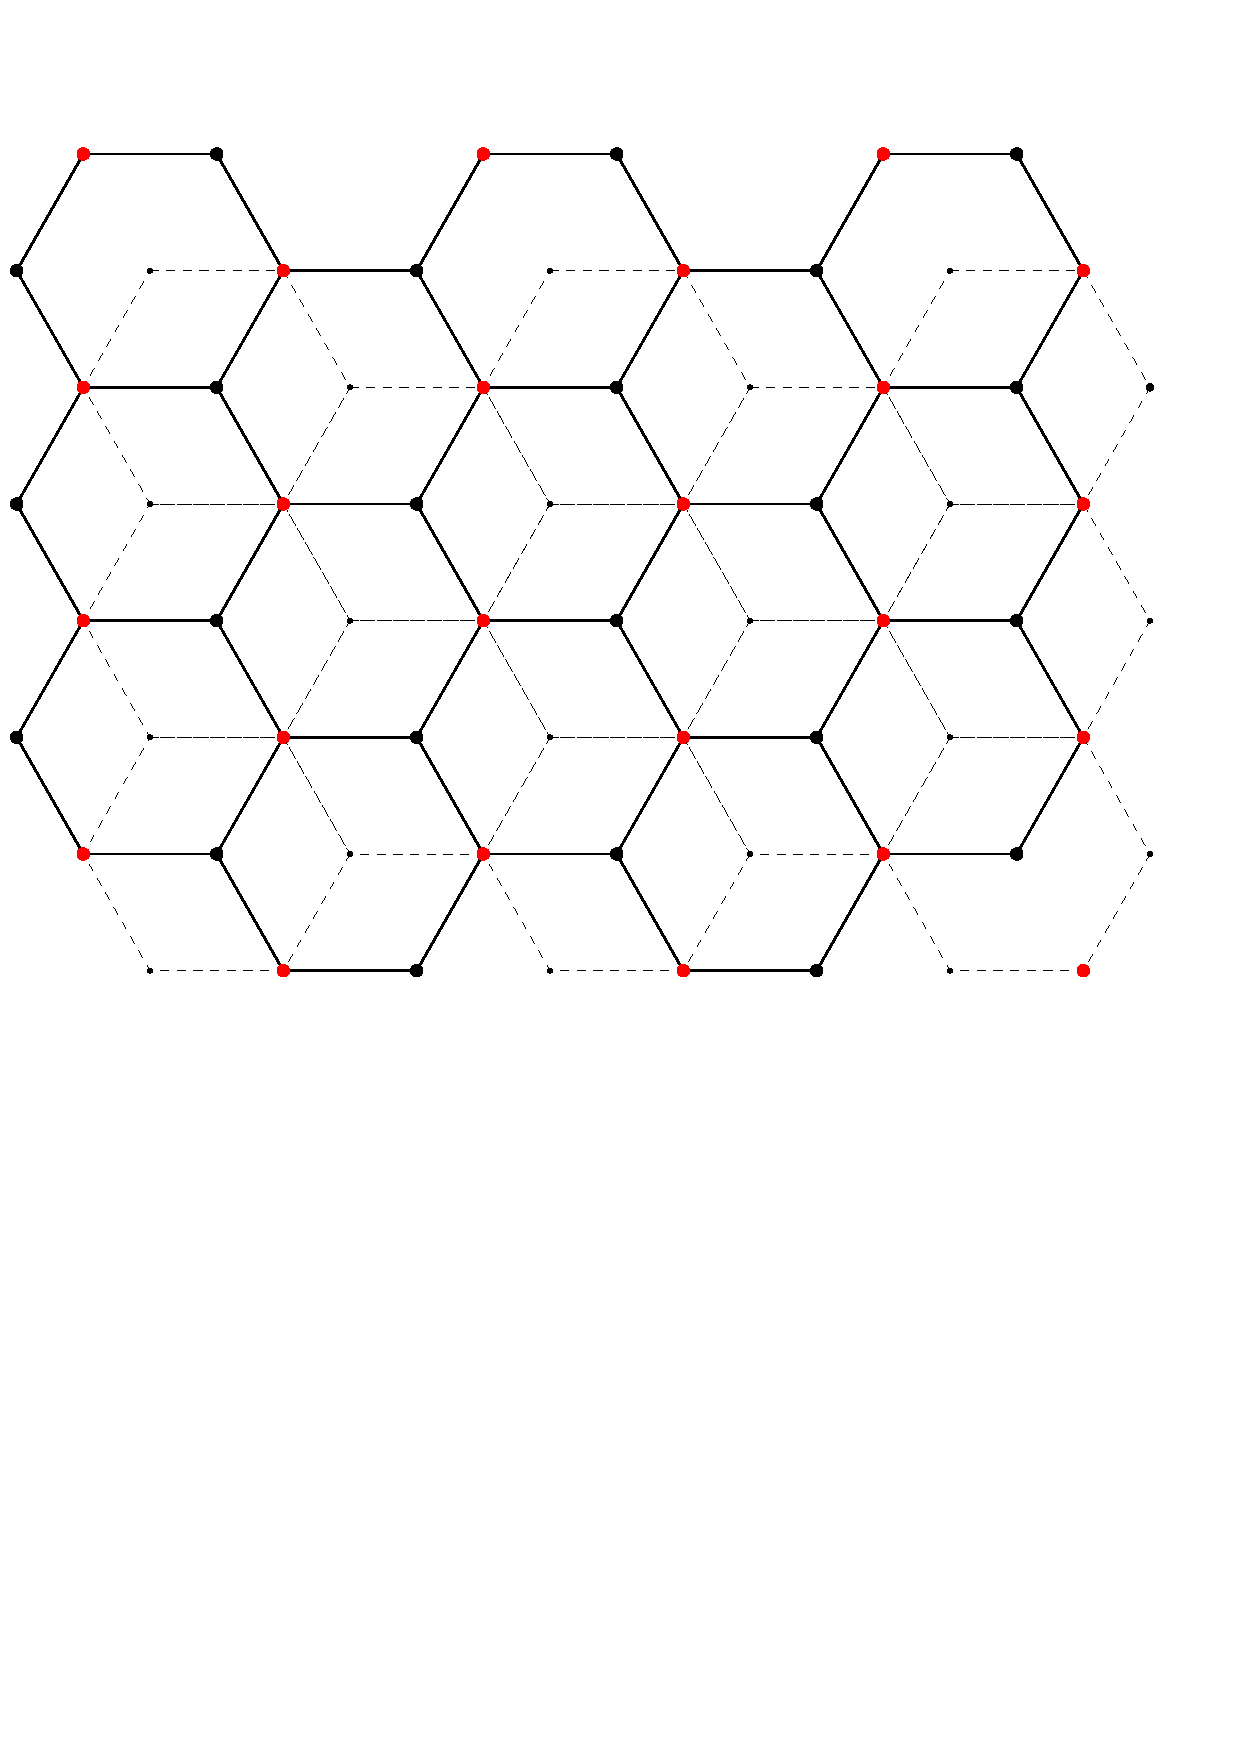
\includegraphics[width=0.7\textwidth]{grafiken/graphit.pdf}
  \caption{Versatz der Graphen-Ebenen in Graphit. Kohlenstoffatome in rot überlappen in den beiden obersten Ebenen}
\end{figure}
Graphit besteht aus geschichteten Ebenen von Kohlenstoff, welcher eine hexagonale Ringstruktur aufweist. 

\subsection{Verwandte Rastermethoden}

\section{Versuchsdurchführung}

\section{Messdaten}

\section{Auswertung}

\section{Diskussion}

\section{Zusammenfassung}

% BIBLIOGRAPHIE

% Maximale Anzahl der Einträge in Klammer
% Zitieren mit \cite{lamport94}
\begin{thebibliography}{9}

% Beispiel
\bibitem{binning}
  G. Binning et al.,
  \emph{Surface Studies by Scanning Tunneling Microscopy},
  Phys. Rev. Lett. 49, 57 (1982).

\bibitem{colton}
  R. J. Colton, A. Engel, J. E. Frommer et al.,
  \emph{Procedures in Scanning Probe Microscopies},
  John Wiley 1998.
  
\end{thebibliography}

\end{document}
